\begin{wrapfigure}[0]{r}[9pt]{0cm}
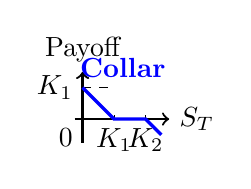
\begin{tikzpicture}[scale=1]
    % --- 定义坐标和参数 ---
    \def\Kone{0.4}       % 行权价 K1 (较低)
    \def\Ktwo{0.8}       % 行权价 K2 (较高, K2 > K1)
    \def\maxST{1}      % S_T 的最大显示范围
    \def\minPayoff{-0.2} % Y轴负半轴的显示范围

    % --- 绘制坐标轴 ---
    % Y 轴 (Payoff) - 需要覆盖正负两个区域
    \draw[->, thick] (0, \minPayoff - 0.1) -- (0, \Kone + 0.2) node[above] {Payoff};
    % X 轴 (S_T)
    \draw[->, thick] (-0.1, 0) -- (\maxST + 0.1, 0) node[right] {$S_T$};

    % --- 绘制辅助线和标签 ---
    % 标记原点
    \node[below left] at (0, 0) {0};

    % 在 X 轴上标记 K1
    \draw (\Kone, 0) node[below] {$K_1$} -- (\Kone, 0.05);

    % 在 X 轴上标记 K2
    \draw (\Ktwo, 0) node[below] {$K_2$} -- (\Ktwo, 0.05);

    % 在 Y 轴正半轴上标记最大收益 K1
    \draw (0, \Kone) node[left] {$K_1$} -- (0.05, \Kone);
    % 从 (0, K1) 向右画水平虚线
    \draw[dashed, thin] (0, \Kone) -- (\Kone, \Kone);
    % 从 (K1, K1) 向下画垂直虚线到 X 轴 (虽然点在轴上, 但为了视觉完整性可以加上)
    %\draw[dashed, thin] (\Kone, 0) -- (\Kone, \Kone);


    % --- 绘制 Collar 收益曲线 (蓝色粗线) ---
    % 路径分析:
    % 1. S_T < K1: 收益为 K1 - S_T。从 (0, K1) 线性下降到 (K1, 0)。
    % 2. K1 <= S_T < K2: 收益为 0。从 (K1, 0) 水平延伸到 (K2, 0)。
    % 3. S_T >= K2: 收益为 K2 - S_T。从 (K2, 0) 开始以斜率 -1 下降。
    %    为了画出最后一段，我们计算一个终点：当 S_T = maxST 时，Payoff = K2 - maxST
    \draw[blue, very thick] (0, \Kone) -- (\Kone, 0) -- (\Ktwo, 0) -- (\maxST, \Ktwo - \maxST);

    % --- 添加标题标签 ---
    % 将标题放在图像的右上方
    \node[blue, anchor=south east, font=\bfseries,xshift=5pt] at (\maxST, \Kone) {Collar};

\end{tikzpicture}
\end{wrapfigure}